\documentclass{article}
\usepackage[utf8]{inputenc}
\usepackage{amsmath}
\usepackage{amssymb}
\usepackage{amsthm}
\usepackage{cancel}
\usepackage[shortlabels]{enumitem}
\usepackage{caption}
\usepackage{graphicx}
\usepackage[top=0.5in, bottom=0.5in, left=1in, right=1in]{geometry}
\usepackage{float}

\title{\textbf{\underline{MATH3090U: Network Science}\\Take Home Exam}}
\author{Syed Naqvi\\100590852}
\date{\today}

\begin{document}

    \maketitle
    
    \subsection*{1.}

    \begin{enumerate}[label=(\alph*), left=10pt, itemsep=10pt]
        
        \item \begin{minipage}[t]{0.9\textwidth}
            Importing data and creating Canadian Airport Network using networkx:
            \begin{figure}[H]
                \centering
                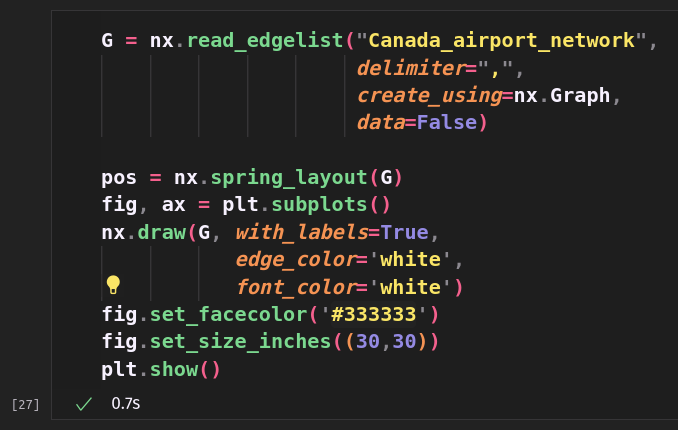
\includegraphics[width=0.8\textwidth, height=0.3\textheight]{./1a.png}
                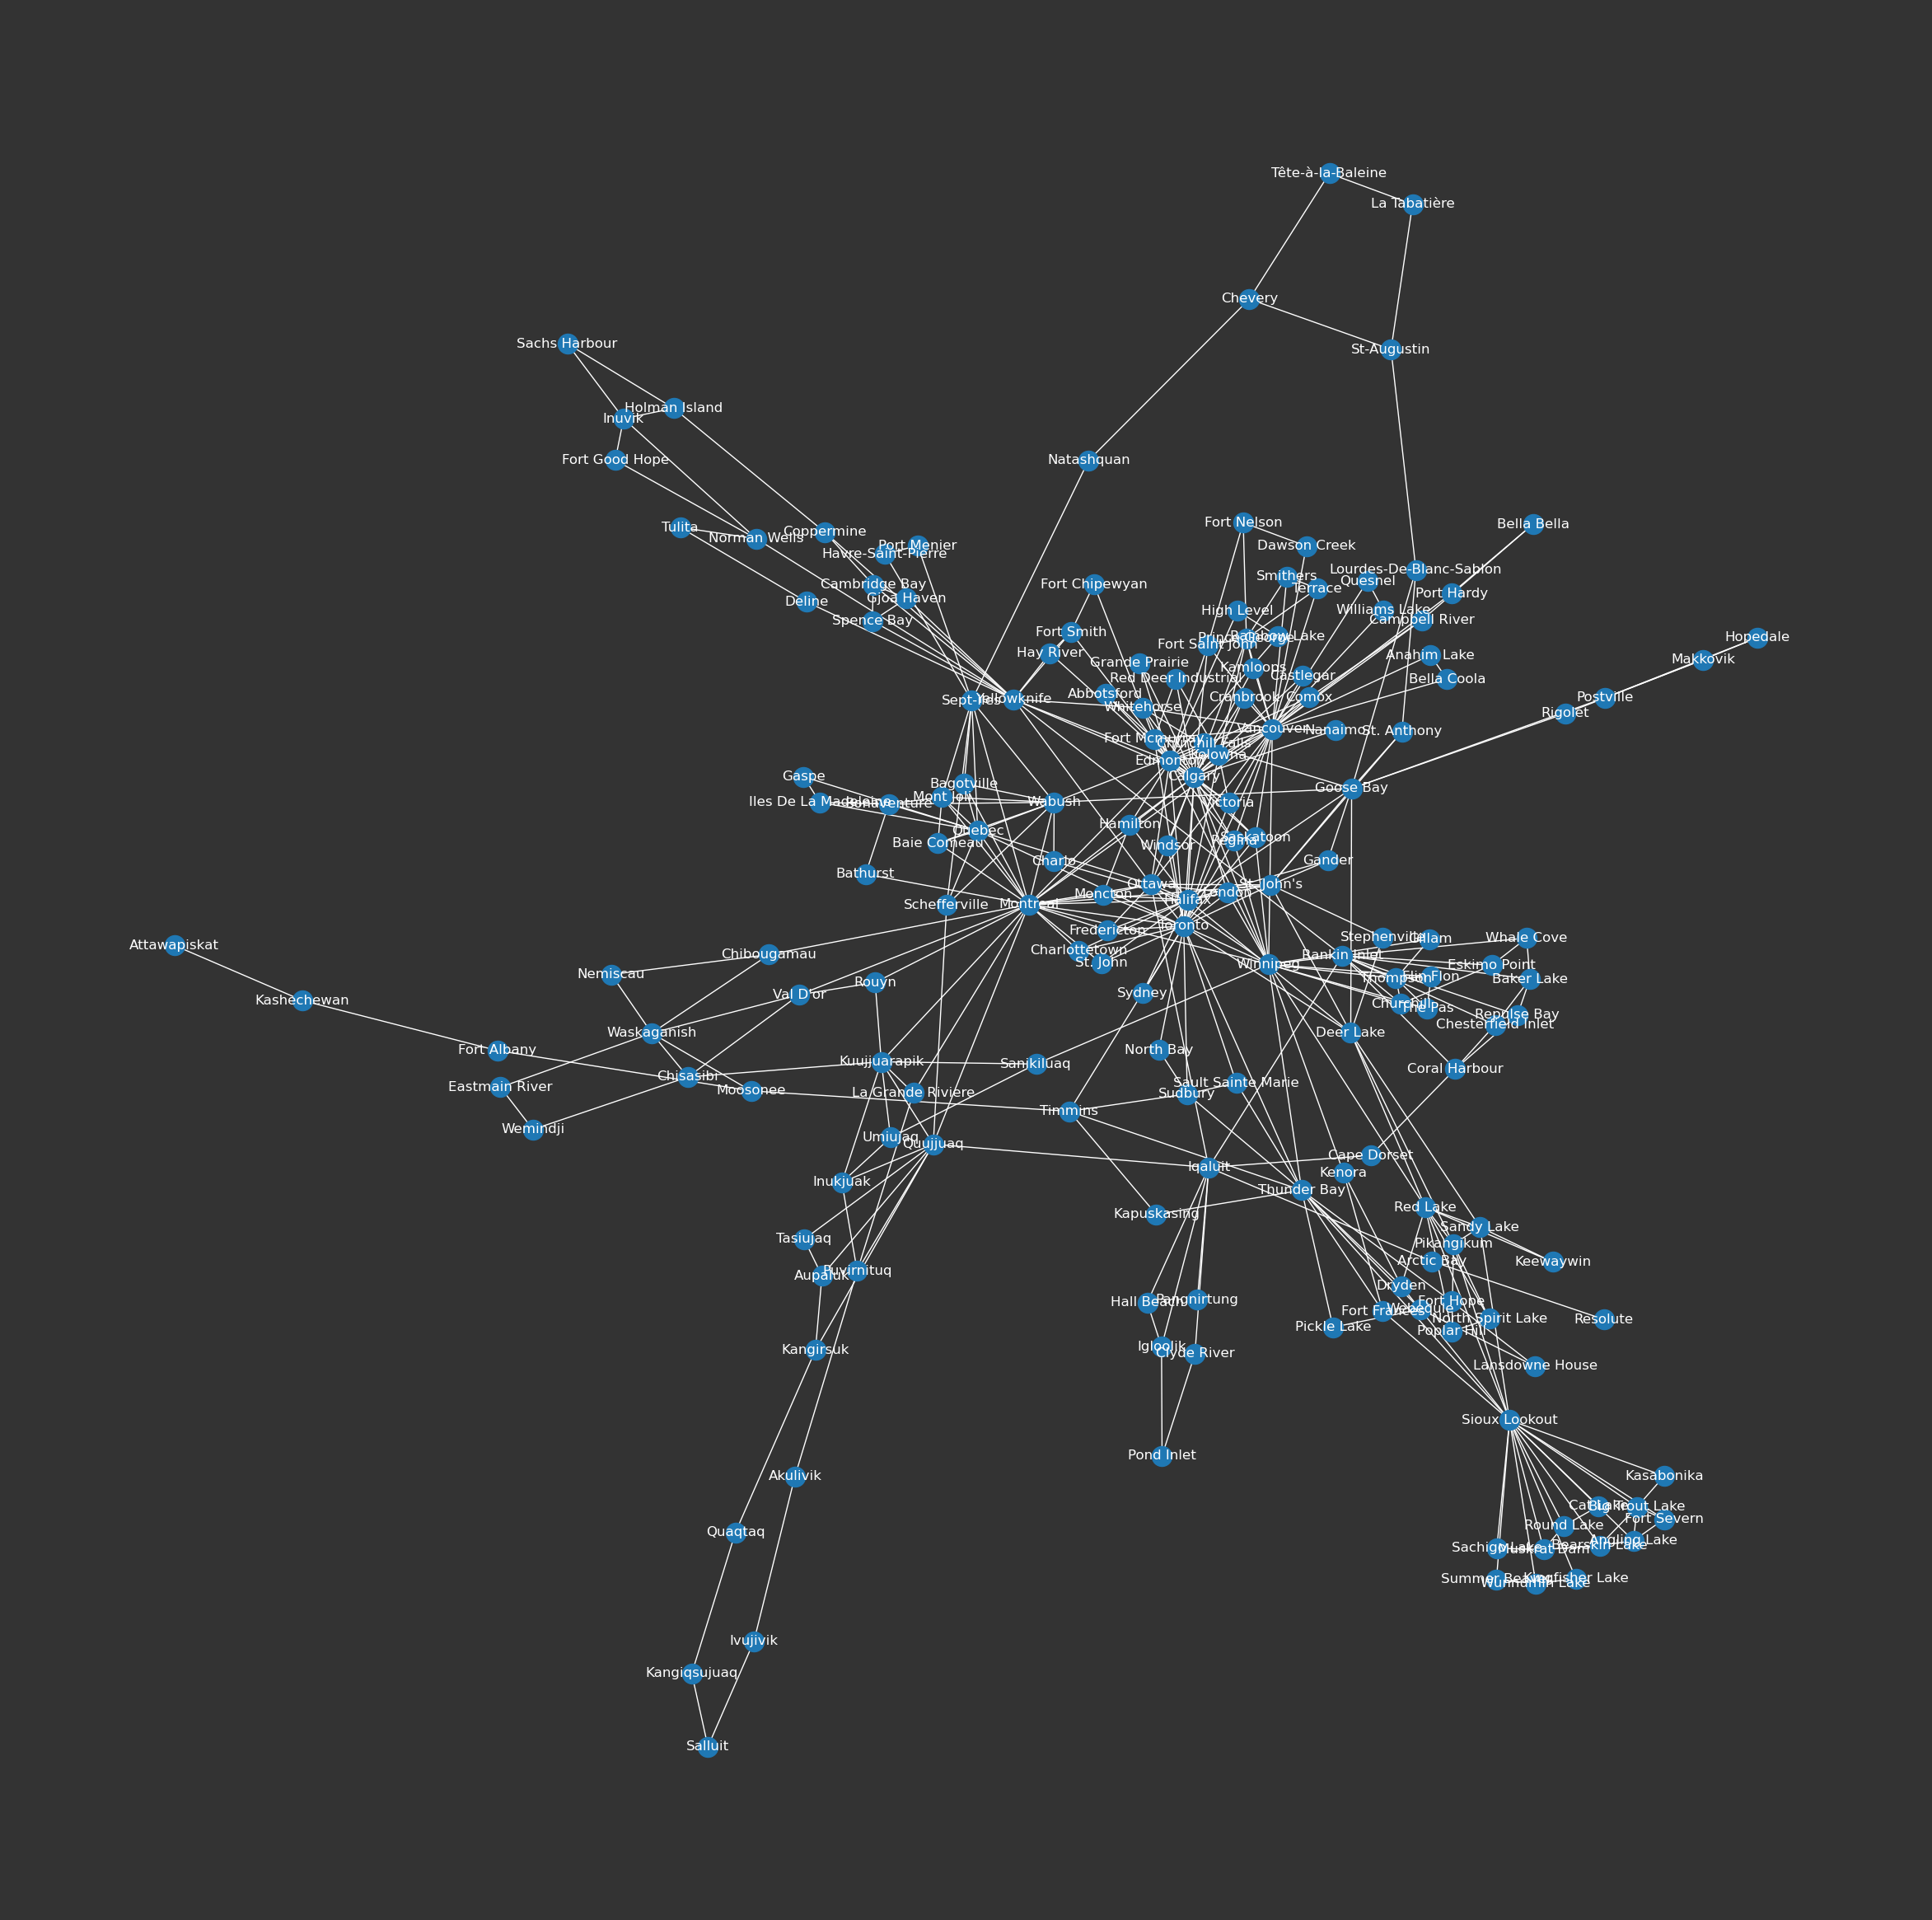
\includegraphics[width=1\textwidth, height=0.4\textheight]{./1ai.png}
            \end{figure}
        \end{minipage}
        
        \item \begin{minipage}[t]{0.9\textwidth}
            Degree distribution histogram and top ten airports(nodes) in terms of degree:
            \begin{figure}[H]
                \centering
                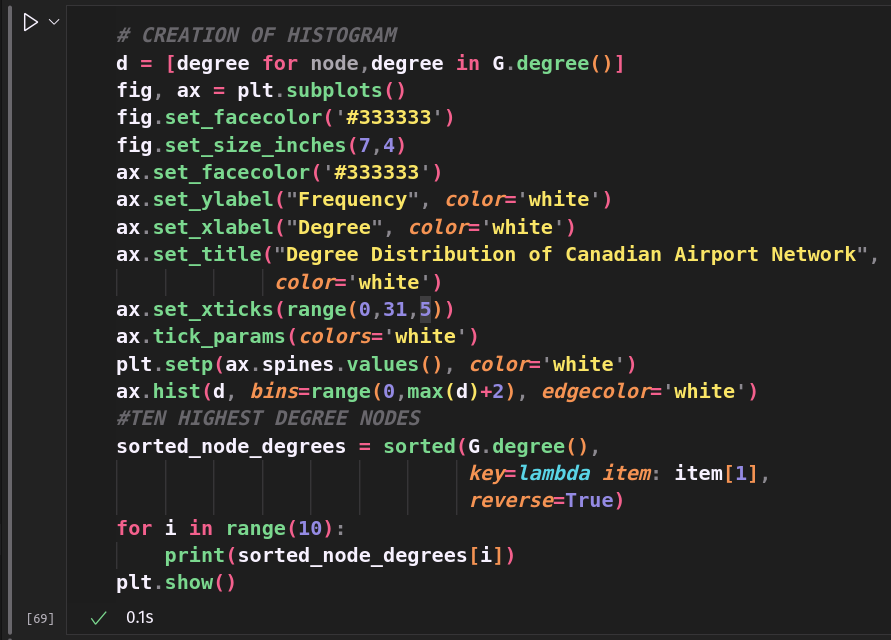
\includegraphics[width=0.8\textwidth, height=0.3\textheight]{./1b.png}
                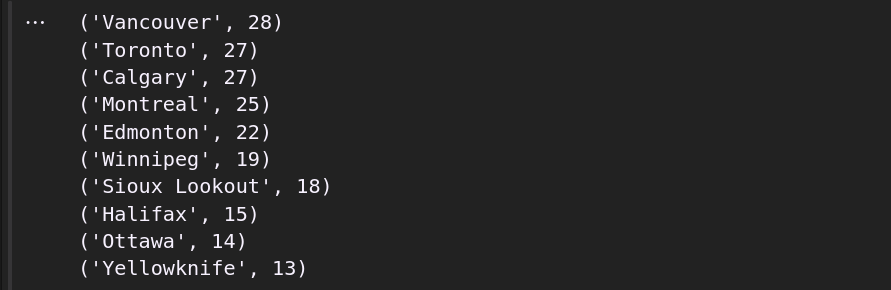
\includegraphics[width=0.8\textwidth, height=0.15\textheight]{./1bi.png}
                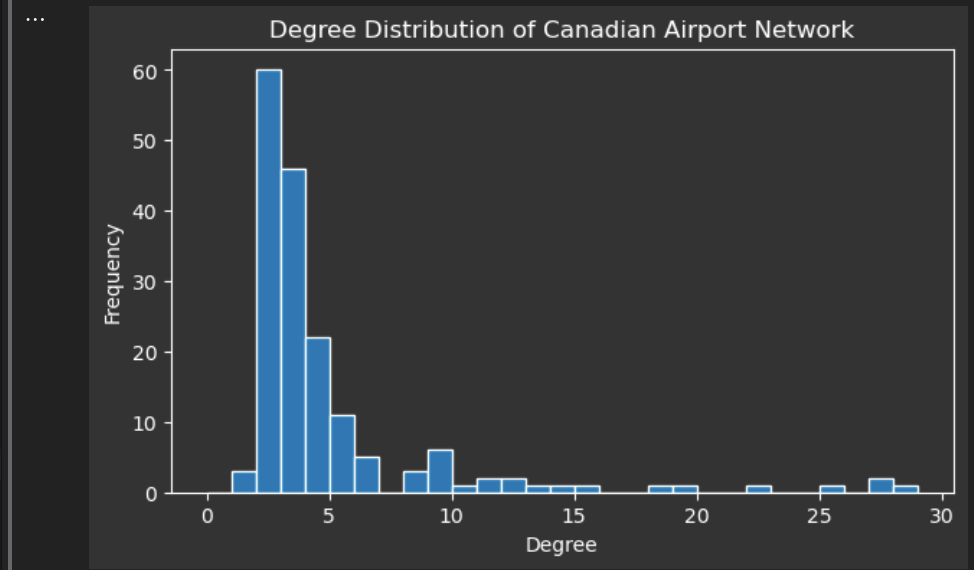
\includegraphics[width=0.8\textwidth, height=0.3\textheight]{./1bii.png}
            \end{figure}
            Sioux lookout Airport being on this list was slighlty surprising as it has 18 connections to
            other airports yet does not reside in a major Canadian city like many of the other nodes on the list.
            After some research it turns out that Sioux Lookout is sometimes referred to as the "Gateway to the North"
            and serves as a hub for providing essential services and connections to many remote first nations
            communities in Northwestern Ontario.
        \end{minipage}

        \item \begin{minipage}[t]{0.9\textwidth}
            Nodes with top ten closeness centralities:
            \begin{figure}[H]
                \centering
                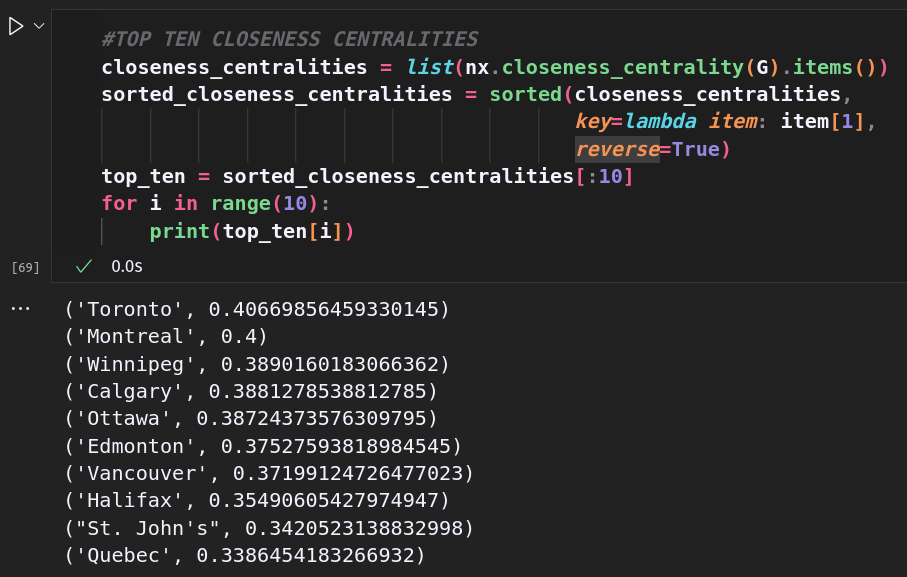
\includegraphics[width=0.8\textwidth, height=0.3\textheight]{./1c.png}
            \end{figure}
        \end{minipage}

        \item \begin{minipage}[t]{0.9\textwidth}
            Nodes with top ten betweenness centralities:
            \begin{figure}[H]
                \centering
                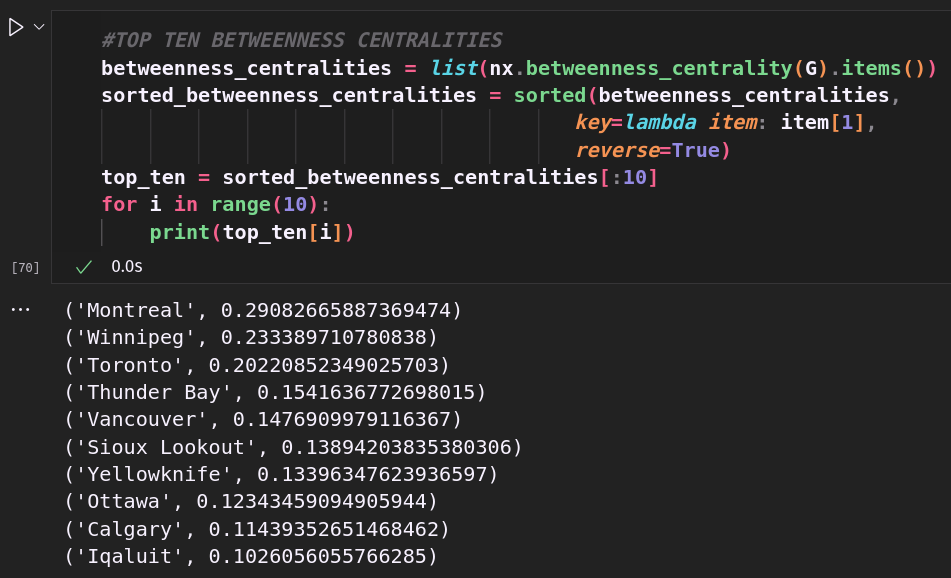
\includegraphics[width=0.8\textwidth, height=0.3\textheight]{./1d.png}
            \end{figure}
        \end{minipage}

        \item \begin{minipage}[t]{0.9\textwidth}
            The airports with the highest degree centrality are those that have the most direct
            connections to other airports. Usually this indicates that the airport is in a large
            metropolitan area but can also indicate a central hub that serves as a connection
            point for many surrounding airports such as with Sioux Lookout.\\

            The closeness centrality is a better indication of a "main airport". An airport with
            high closeness centrality is one from which the rest of the country is accessible
            via minimum intermediary stops. Unsurprisingly, the top ten nodes with highest
            closeness centralities are all captial cities or highly populated cities.
            This is to be expected since these are locations most people would be traveling to or
            from and so would be closeset to all other airports.\\

            A high betweenness centrality indicates an airport that sits between different clusters
            of airports. Such airports tend to be on many shortest flight routes between airports
            in opposing parts of the network. We can see this reflected in the fact that most
            airports on the top ten betweenness centrality list are in geographically central parts
            of Canada, thus lying on the shortest flight routes between east and west cost.
            A few others, althout not geographically central, serve as local bottlenecks separating
            smaller clusters from the rest of the network such as Sioux Lookout and Vancouver.
        \end{minipage}

        \item \begin{minipage}[t]{0.9\textwidth}
            Using Girvan Newman Algorithm to determine a parition with highest modularity:
            \begin{figure}[H]
                \centering
                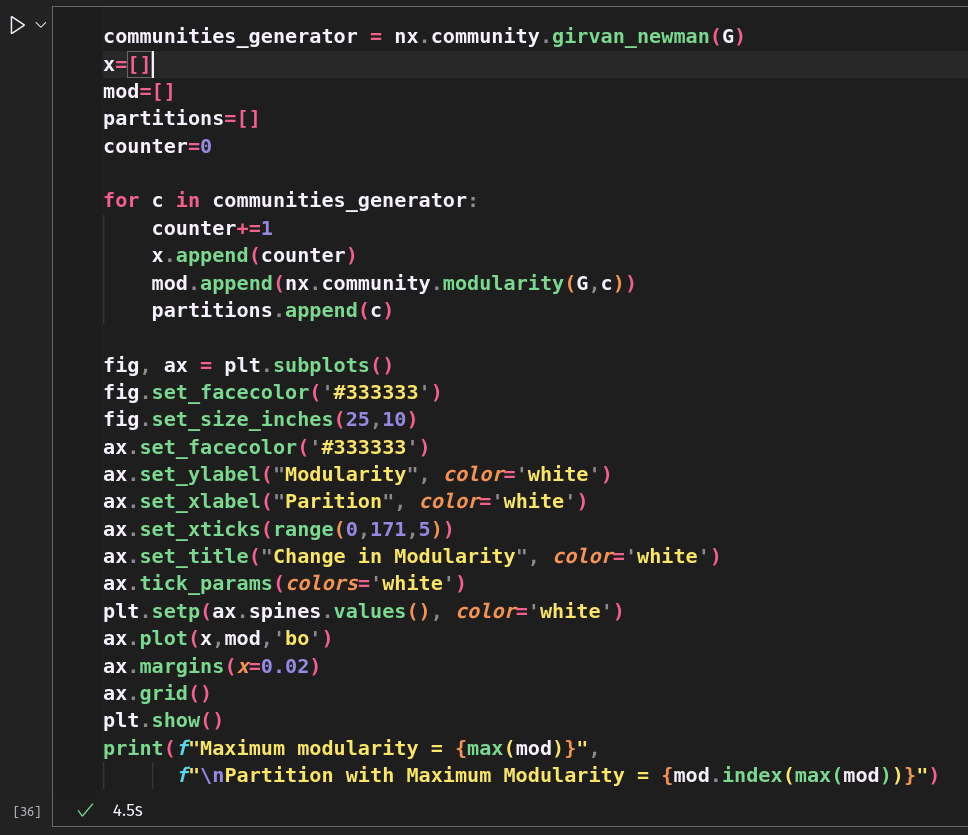
\includegraphics[width=0.8\textwidth, height=0.4\textheight]{./1f.png}
                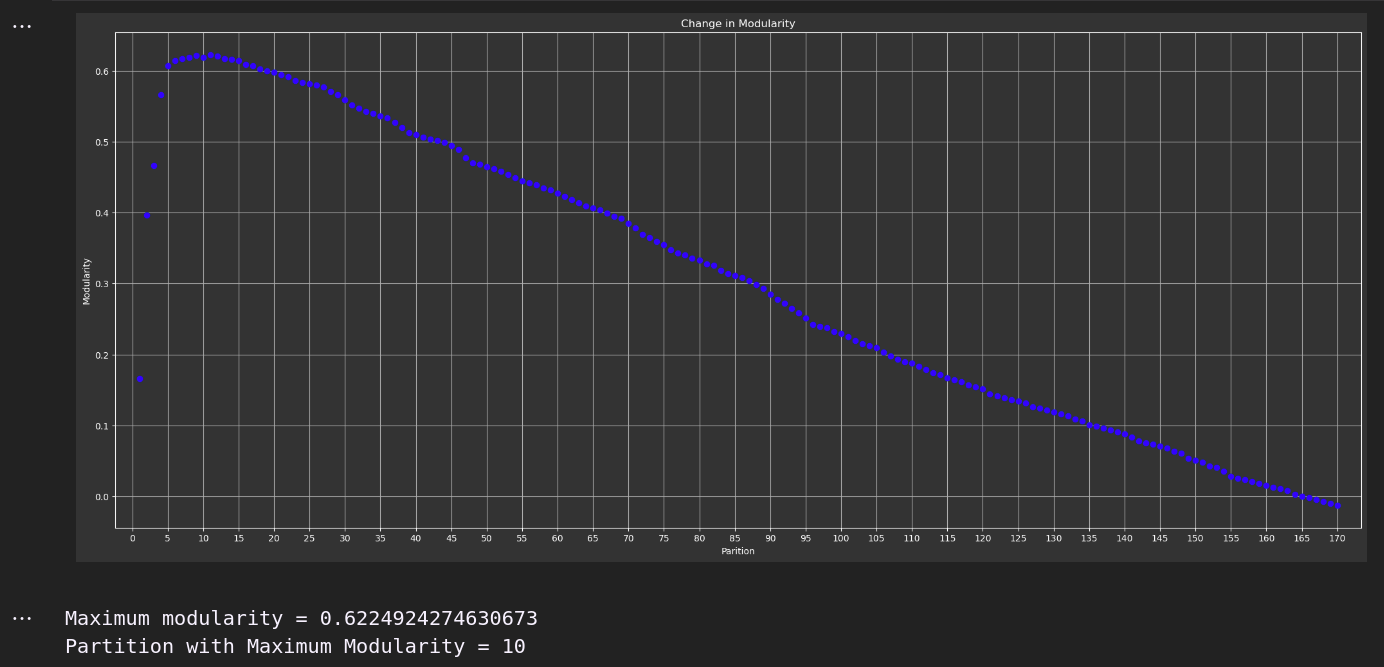
\includegraphics[width=1\textwidth, height=0.3\textheight]{./1fi.png}
            \end{figure}
        \end{minipage}

        \item \begin{minipage}[t]{0.9\textwidth}
            I will be dicussing the community structure from part (f) with the visualization
            presented in this part.
            \begin{figure}[H]
                \centering
                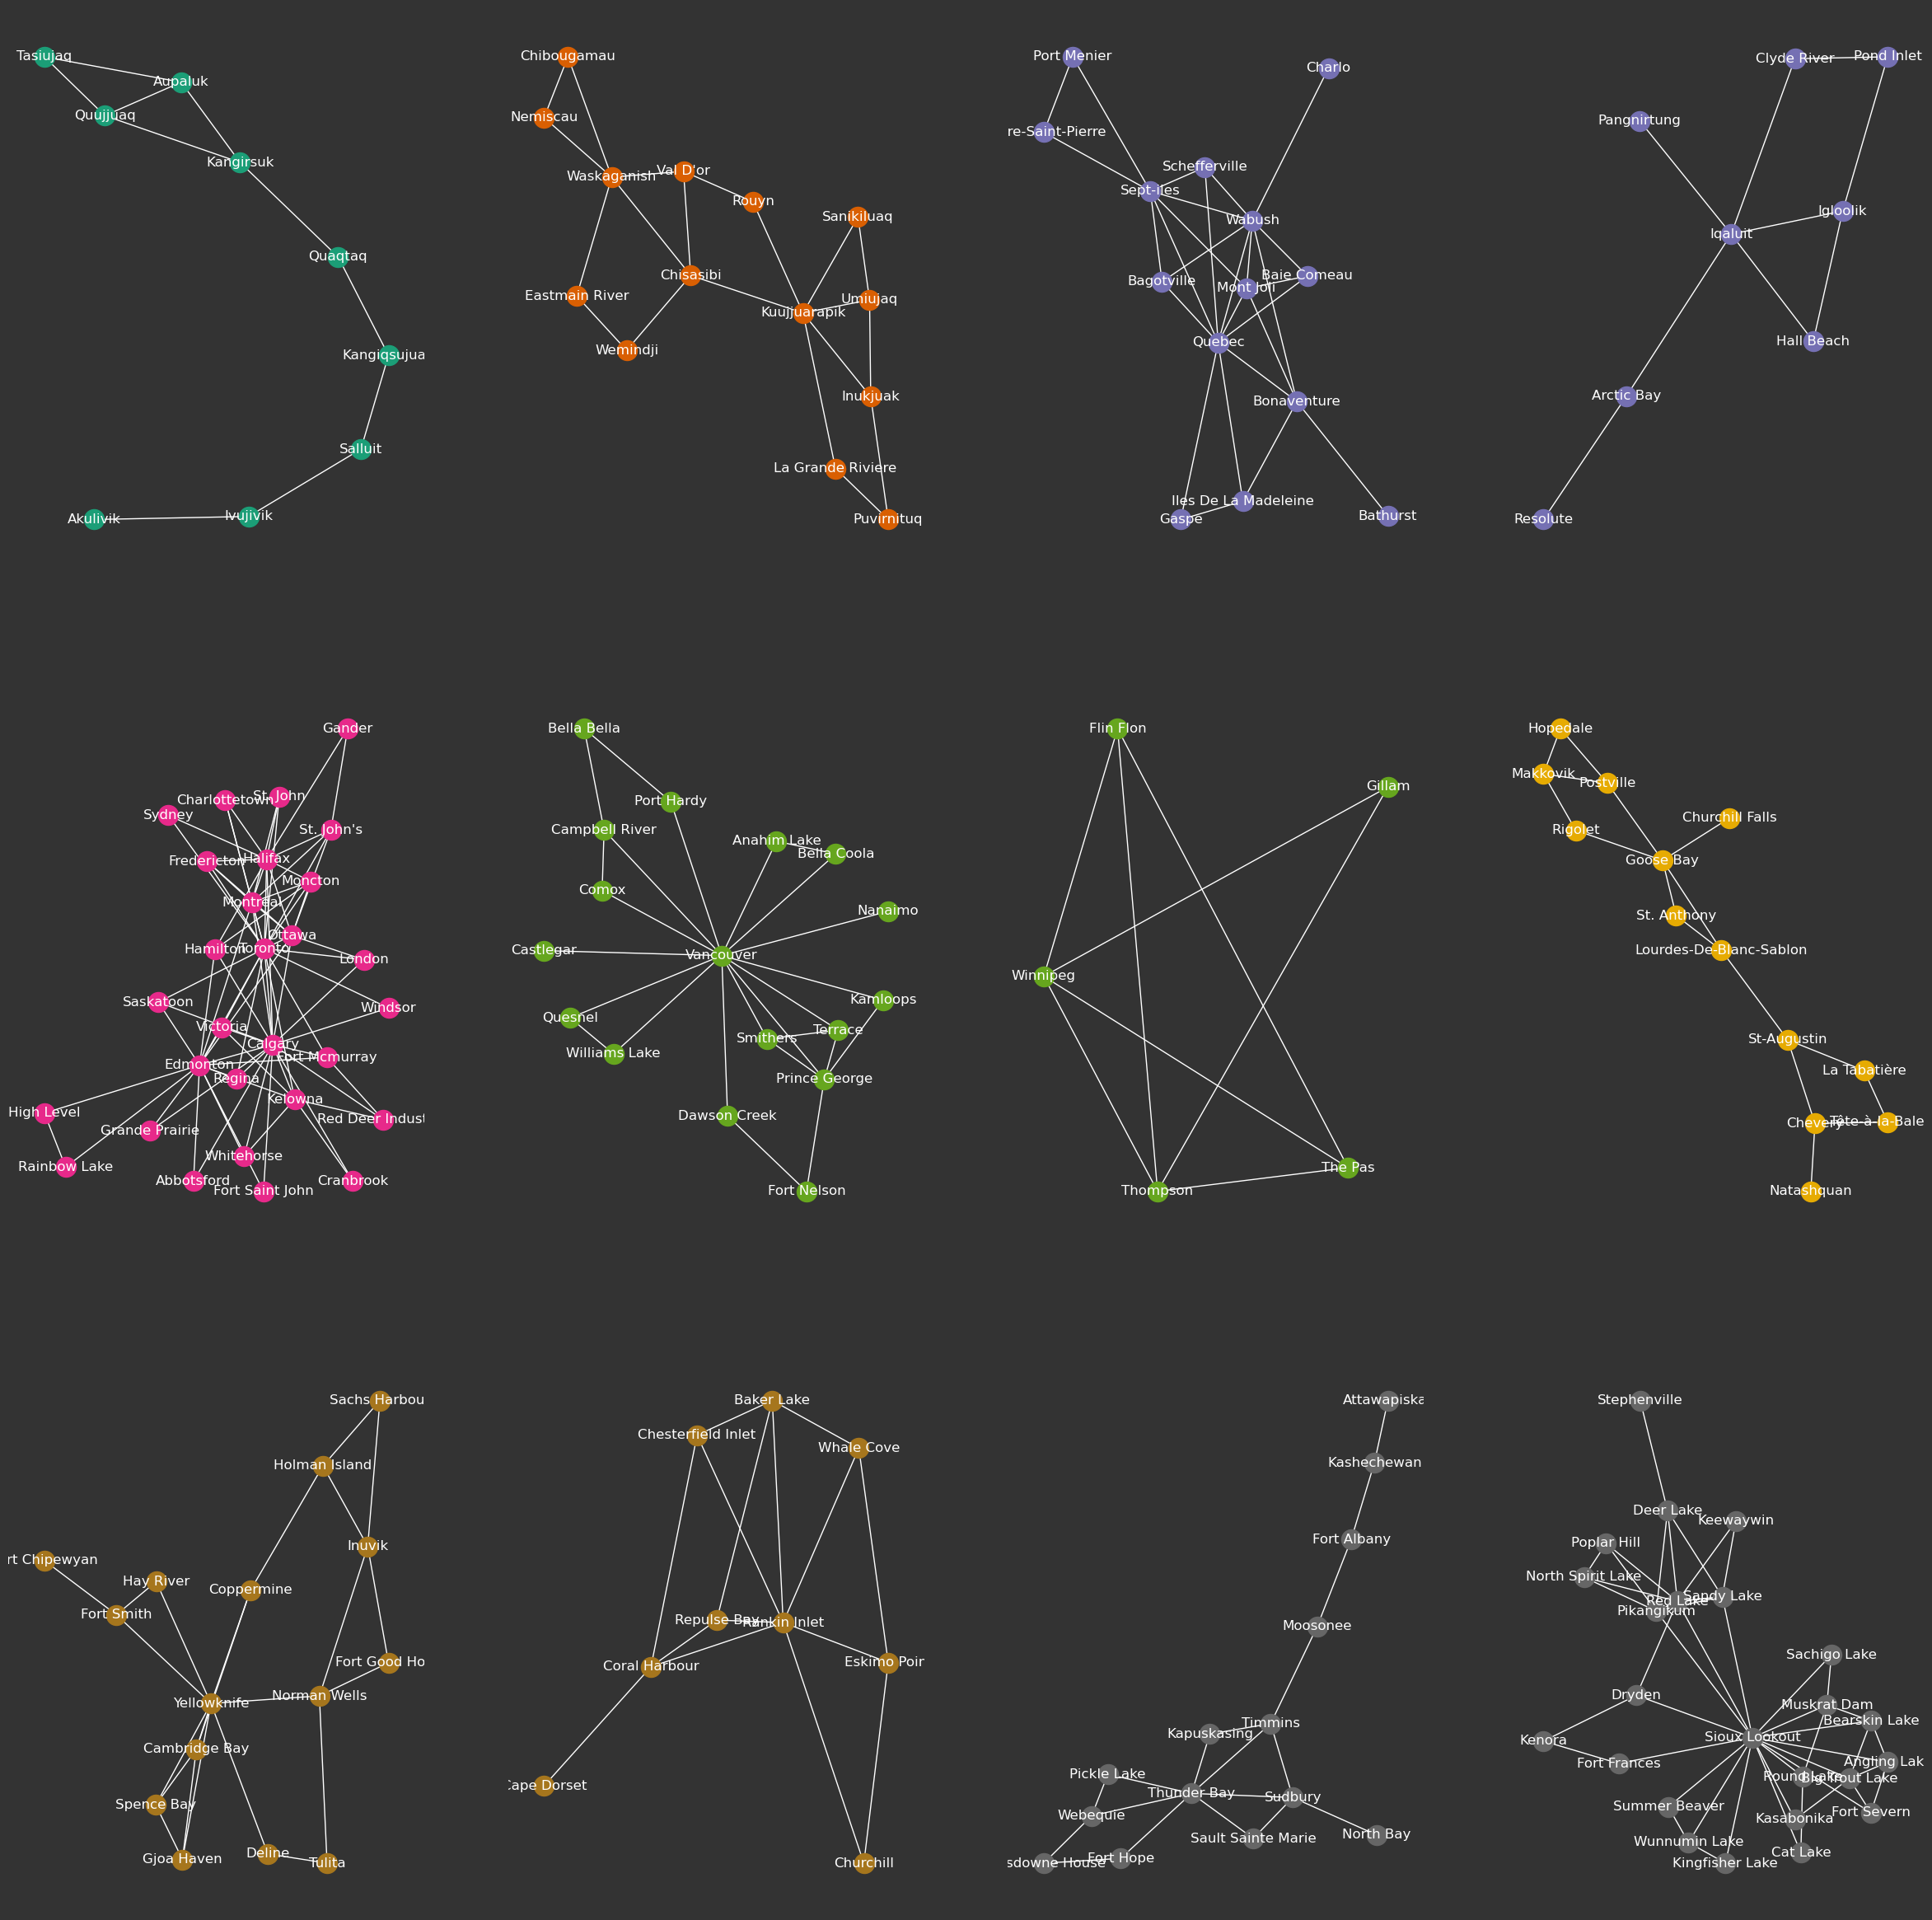
\includegraphics[width=1\textwidth, height=0.5\textheight]{./1g.png}
            \end{figure}
            One notable observation of this network is the strong separation by region and by 
            the strongest hubs. Overall, the communities seem to be split by region likely due
            to the fact that geographically closer airports have more direct flights between
            each other than with other airports in the network. This also makes sense when we
            consider that the Girvan-Newman approach uses betweenness centrality to remove edges
            for each partition and so connection between regions would be removed leaving the
            different regions as distinct communities.\\

            It was also notable that the most central hub airports such as Toronto, Montreal,
            Ottawa, Calgary and their surrounding airports also formed one large community. This is
            probably because of the strong connections between each of these airports leading to
            multiple paths from one of these central airports to their peripheral/regional
            connections resulting in the entirety of this cluster becoming one community.\\

            I think this is a strong visualization as we can clearly see all the communities from
            the parition with the largest modularity score. To create this network, I first stored
            the list of sets of nodes constituting the strongest partition, lets call this
            $P_{best}$. I then iterated through the original graph and removed all edges between
            nodes that did not belong to the same community as determined by $P_{best}$. After
            the graph had been separated into components where each component was a community,
            i then generated 12 subplots, and used nx.draw() to draw each component as a separate
            graph on its own plot out of the 12 subplots. I also colored each plot with a different
            color from the other plots for more readability.
        \end{minipage}

    \end{enumerate}

    \subsection*{2.}

    \begin{enumerate}[label=(\alph*), left=10pt, itemsep=10pt]
        
        \item \begin{minipage}[t]{0.9\textwidth}
            Importing data and creating Social Network using networkx:
            \begin{figure}[H]
                \centering
                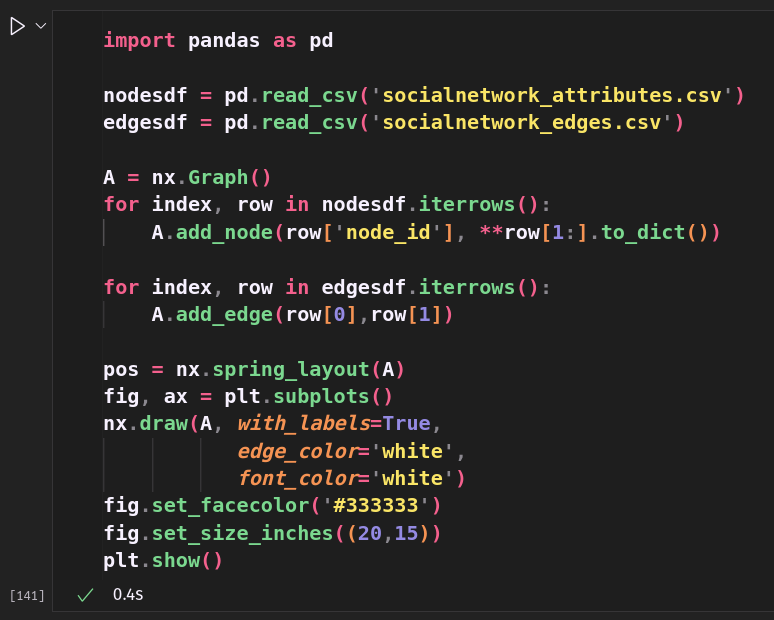
\includegraphics[width=0.8\textwidth, height=0.3\textheight]{./2a.png}
                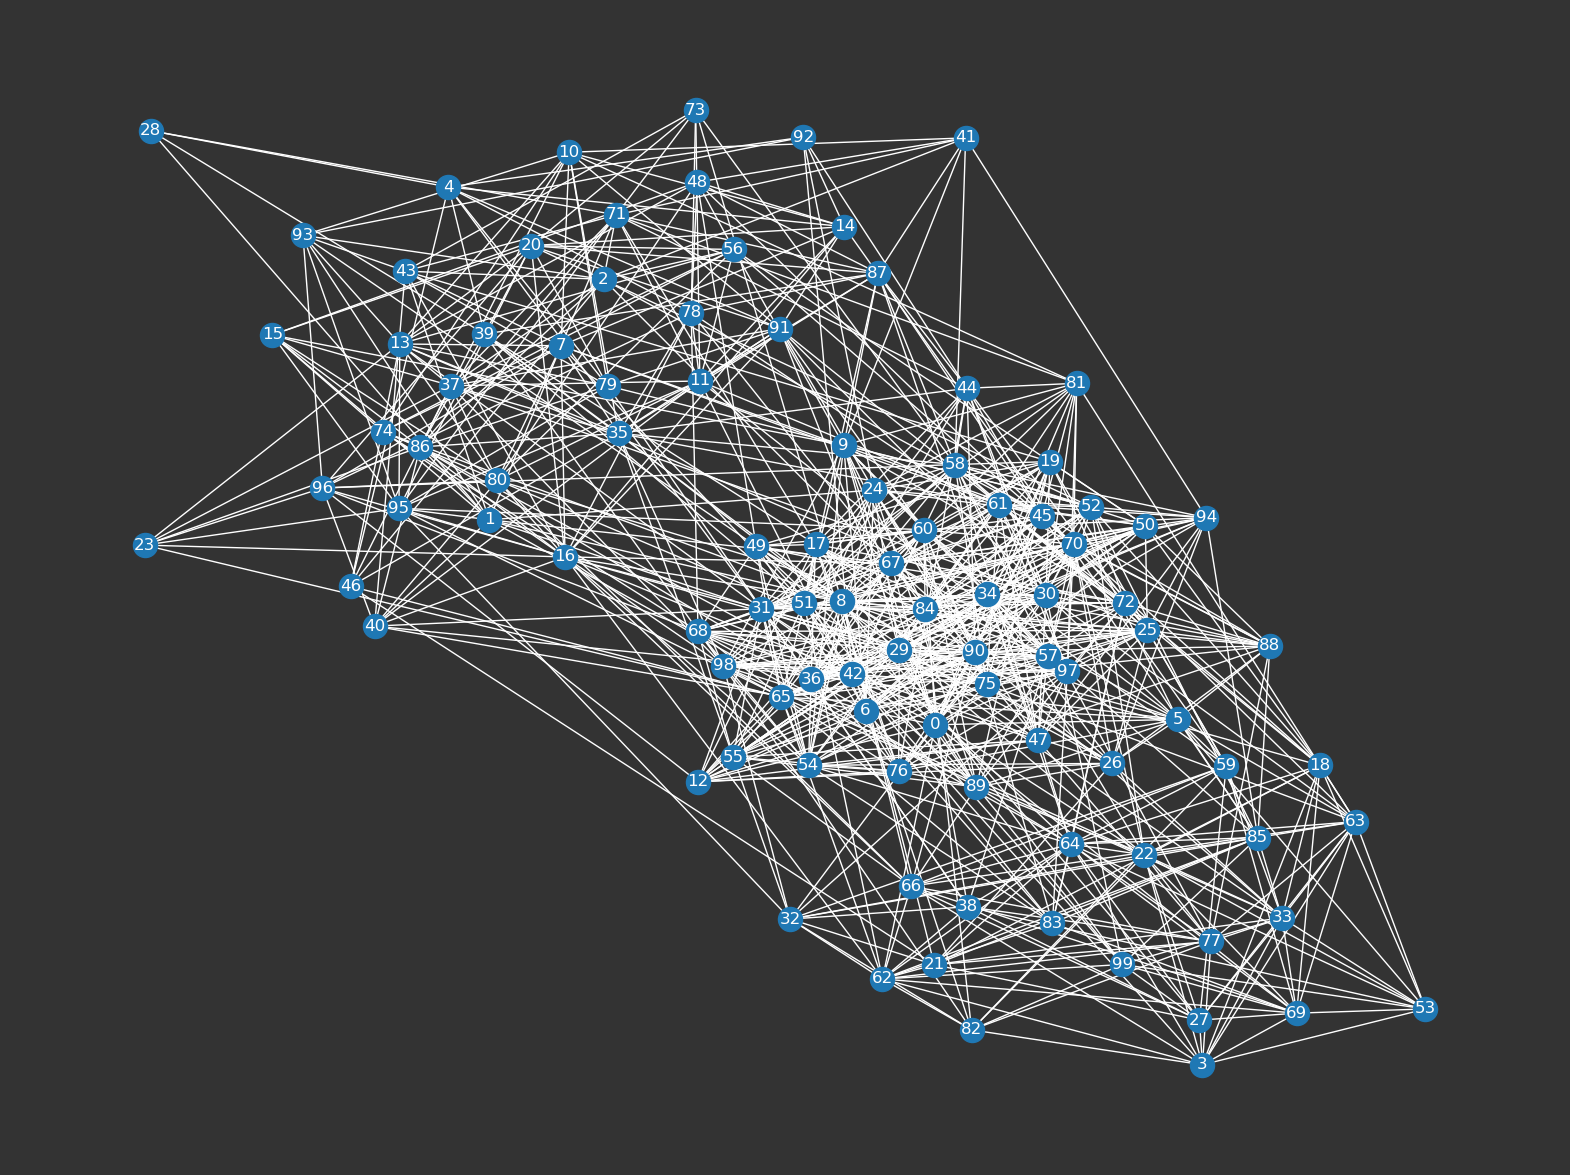
\includegraphics[width=1\textwidth, height=0.4\textheight]{./2ai.png}
            \end{figure}
        \end{minipage}

        \item \begin{minipage}[t]{0.9\textwidth}
            Attributes and possible options:
            \begin{figure}[H]
                \centering
                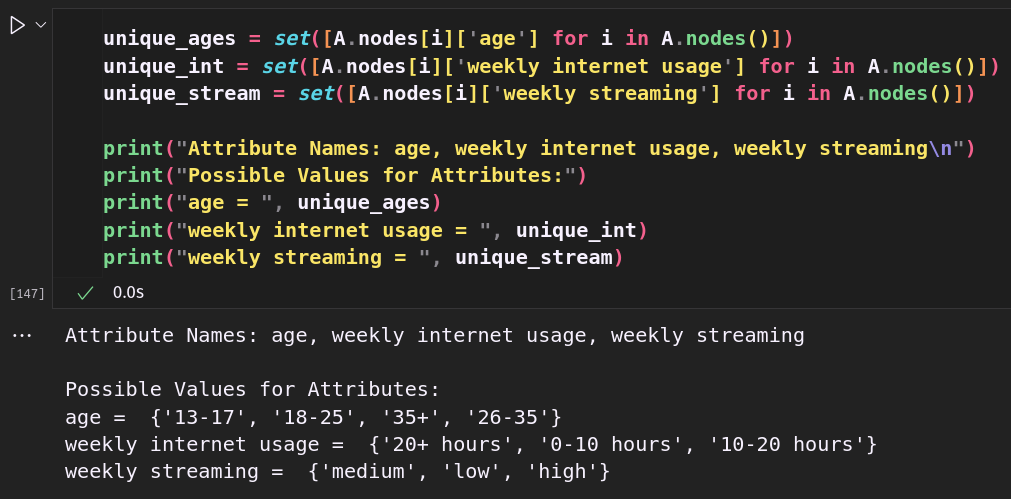
\includegraphics[width=0.9\textwidth, height=0.3\textheight]{./2b.png}
            \end{figure}
        \end{minipage}

        \item \begin{minipage}[t]{0.9\textwidth}
            Attribute value distributions:
            \begin{figure}[H]
                \centering
                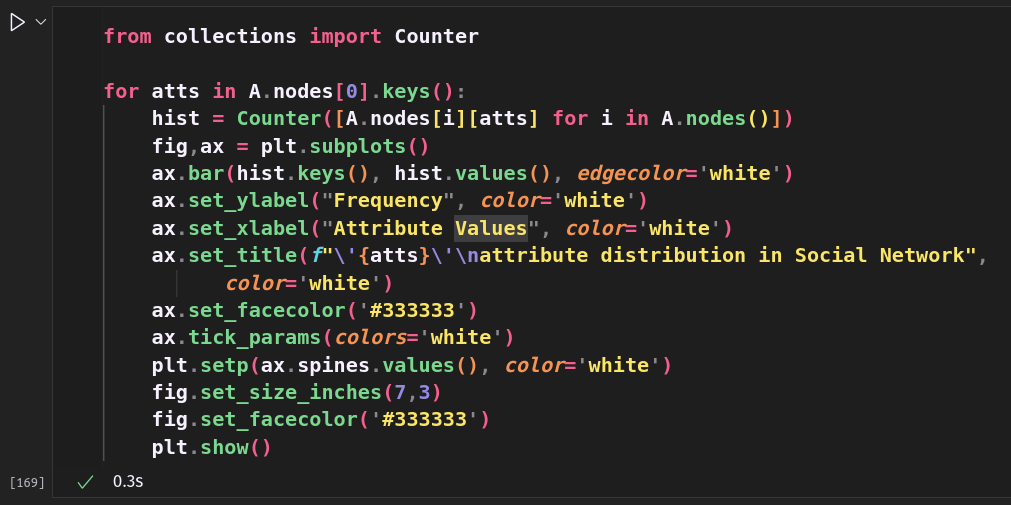
\includegraphics[width=0.9\textwidth, height=0.3\textheight]{./2c.png}
                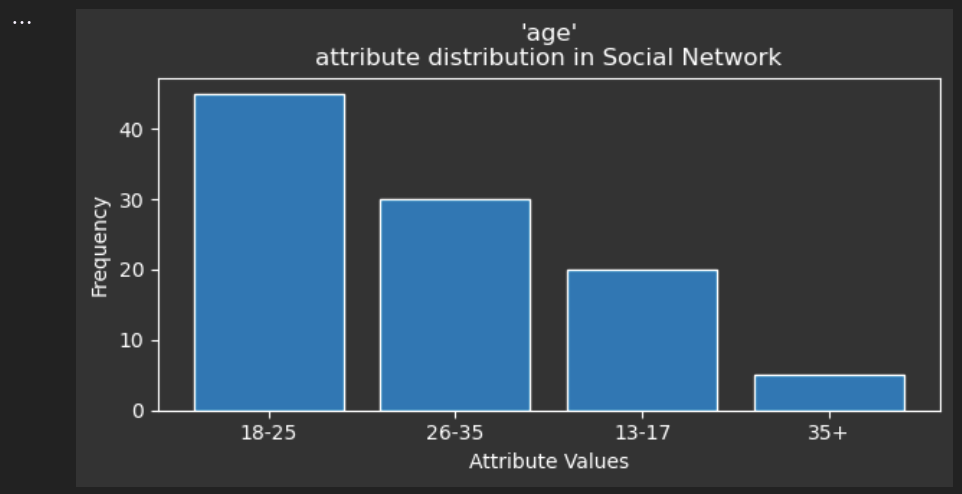
\includegraphics[width=0.9\textwidth, height=0.3\textheight]{./2ci.png}
                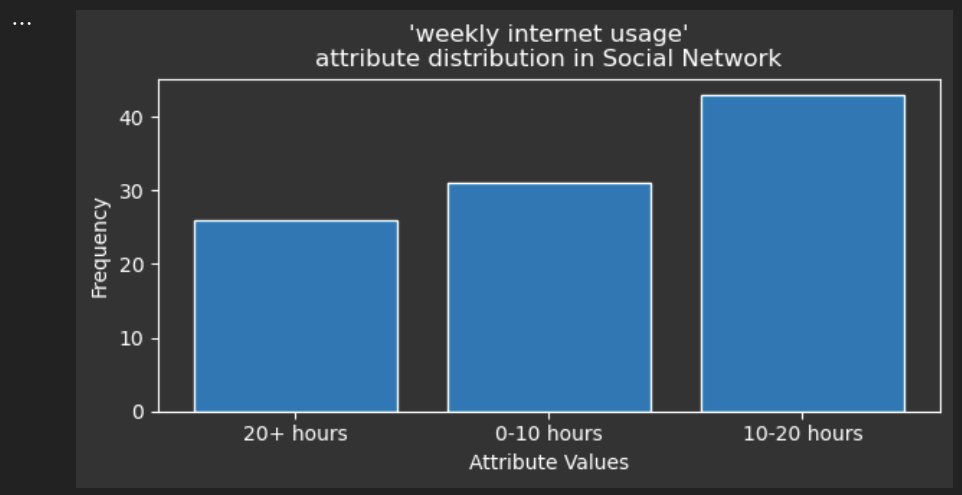
\includegraphics[width=0.9\textwidth, height=0.3\textheight]{./2cii.png}
            \end{figure}
        \end{minipage}
        \newpage
        \begin{minipage}[t]{0.9\textwidth}
            \begin{figure}[H]
                \centering
                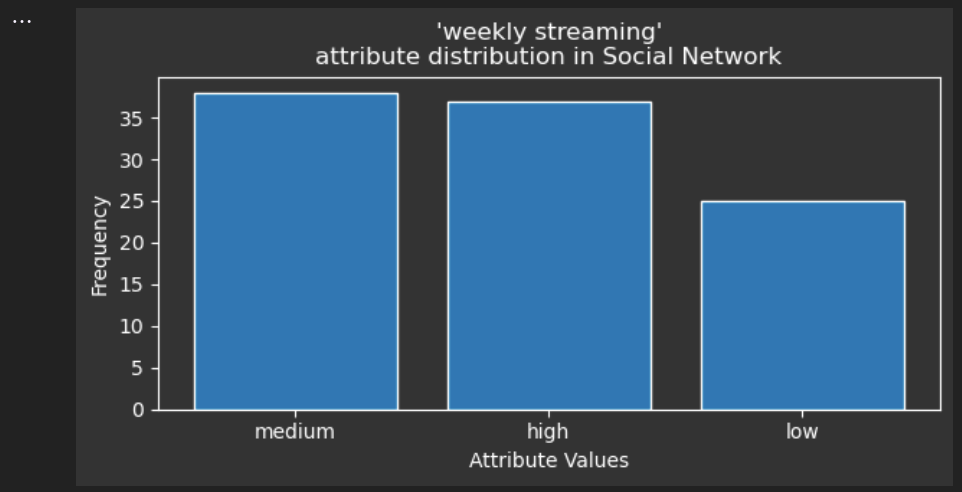
\includegraphics[width=0.9\textwidth, height=0.3\textheight]{./2ciii.png}
            \end{figure}    
        \end{minipage}

        \item \begin{minipage}[t]{0.9\textwidth}
            Modularites based on attribute value partitioning:
            \begin{figure}[H]
                \centering
                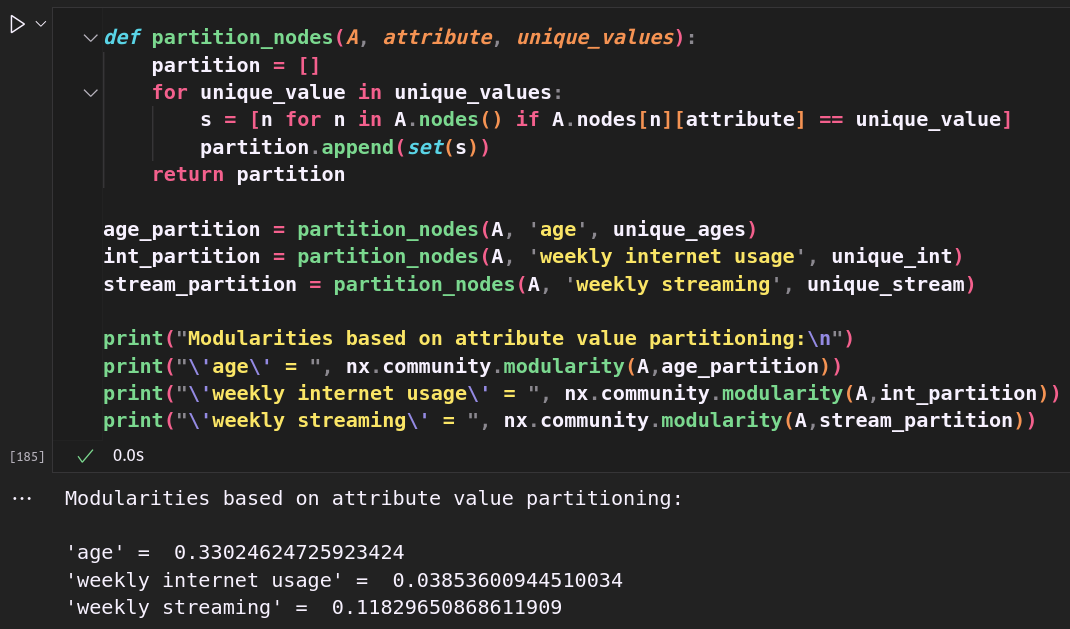
\includegraphics[width=0.9\textwidth, height=0.3\textheight]{./2d.png}
            \end{figure}
        \end{minipage}

        \item \begin{minipage}[t]{0.9\textwidth}
            The findings from part d suggest that people in similar age groups are more likely to
            be friends. If we were to consider a graphical representation of partitioning based
            on the 'age' attribute, we would find that the strongest communities are formed
            amongst nodes in the same age bracket.
        \end{minipage}

        \newpage

        \item \begin{minipage}[t]{0.9\textwidth}
            \begin{figure}[H]
                \centering
                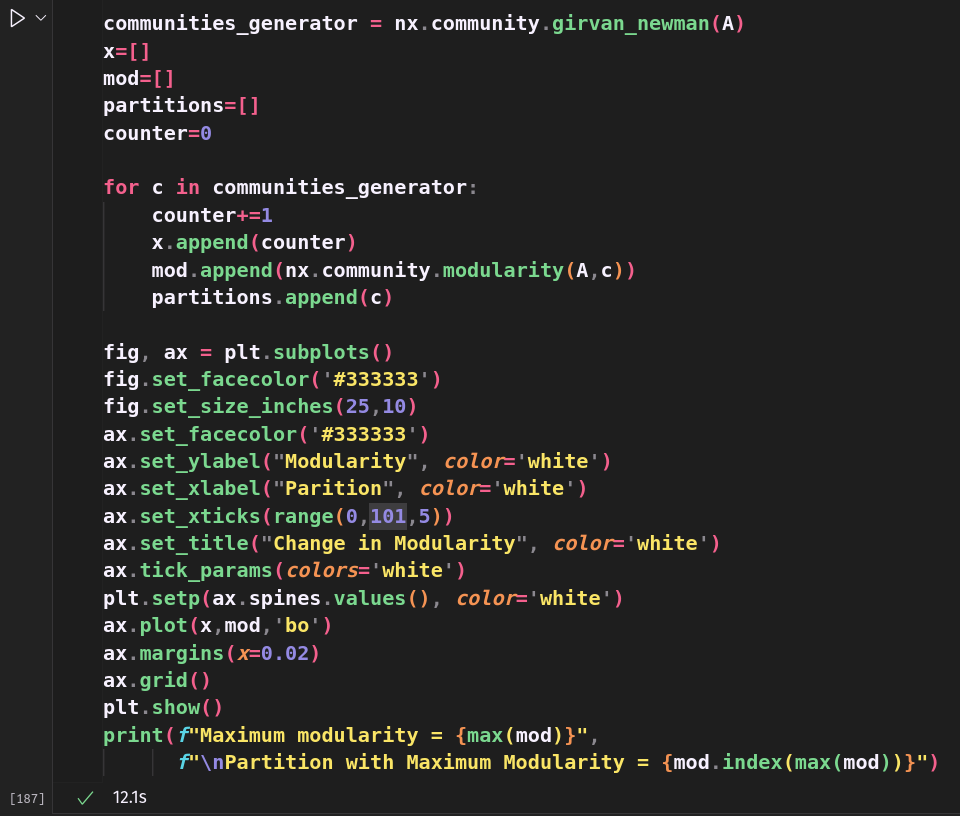
\includegraphics[width=0.9\textwidth, height=0.45\textheight]{./2f.png}
                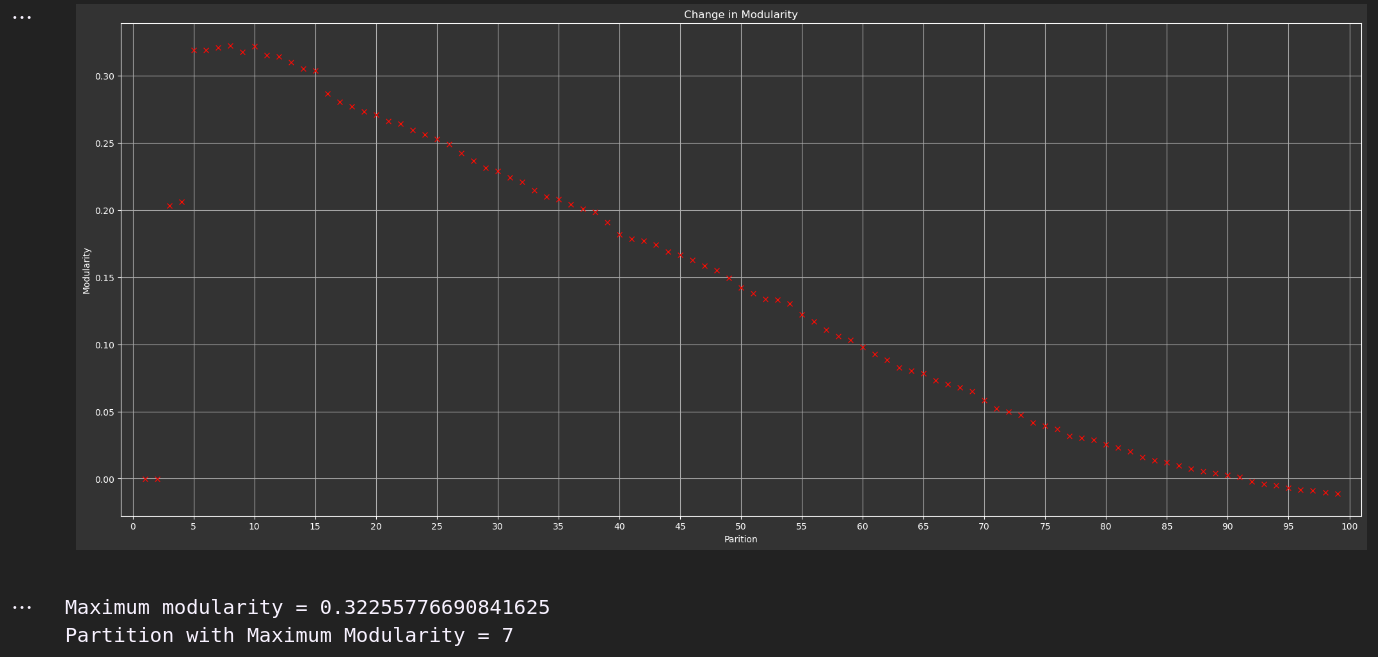
\includegraphics[width=0.9\textwidth, height=0.3\textheight]{./2fi.png}
            \end{figure}
            We observe that using the Girvan-Newman method in order to find the best
            partition of a graph based on modularity may not always capture community structures
            perfectly. Here our best partitioning achieves a maximum modularity of approx
            0.323 which although very close to the partitioning based on age (0.330246)
            is not as high.
        \end{minipage}

        \item \begin{minipage}[t]{0.9\textwidth}
            \begin{figure}[H]
                \centering
                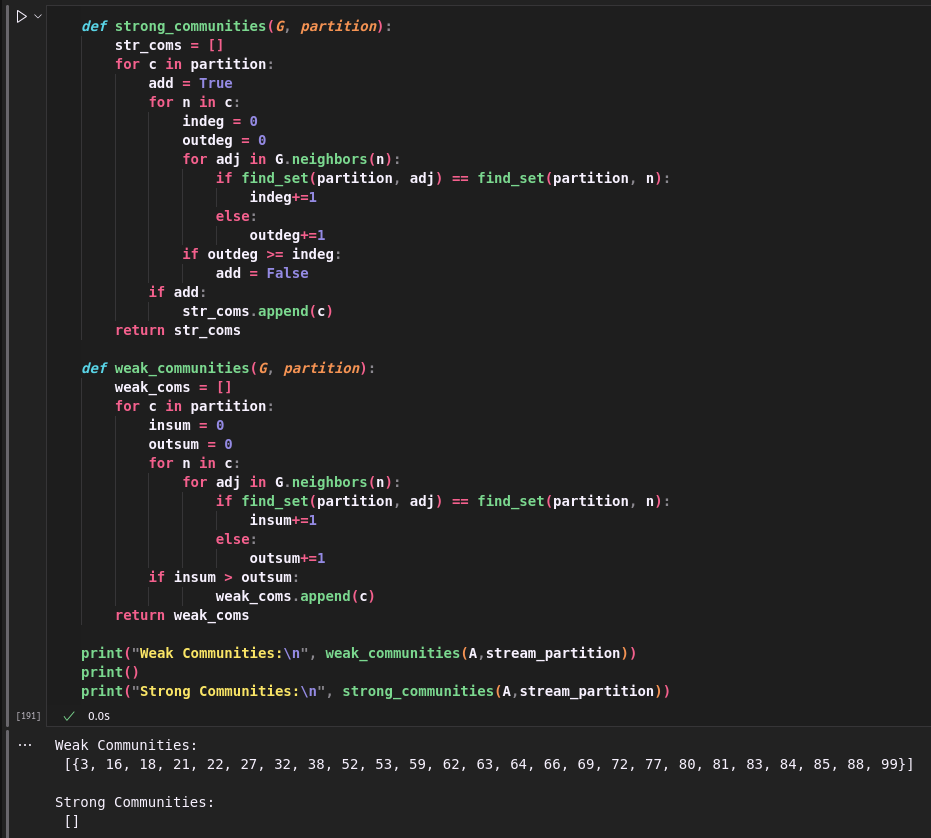
\includegraphics[width=0.9\textwidth, height=0.45\textheight]{./2g.png}
            \end{figure}
            Only one of the subgraphs induced by the streaming usage attribute partition forms
            a weak community and none form a strong community.
        \end{minipage}

    \end{enumerate}


    \subsection*{3.}

    \begin{enumerate}[label=(\alph*), left=10pt, itemsep=10pt]
        
        \item \begin{minipage}[t]{0.9\textwidth}
            Importing data and creating Wiki Page Network using networkx:
            \begin{figure}[H]
                \centering
                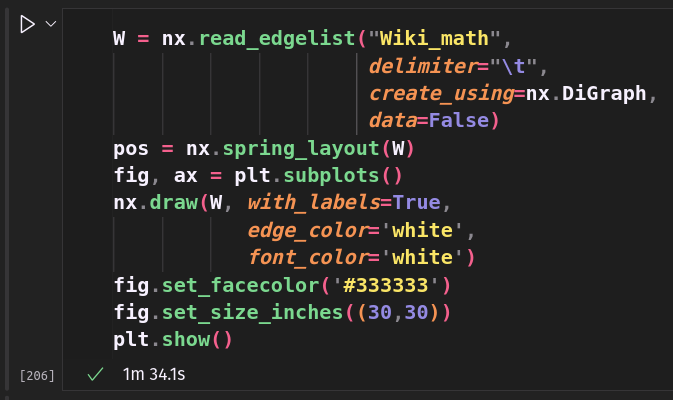
\includegraphics[width=0.8\textwidth, height=0.3\textheight]{./3a.png}
                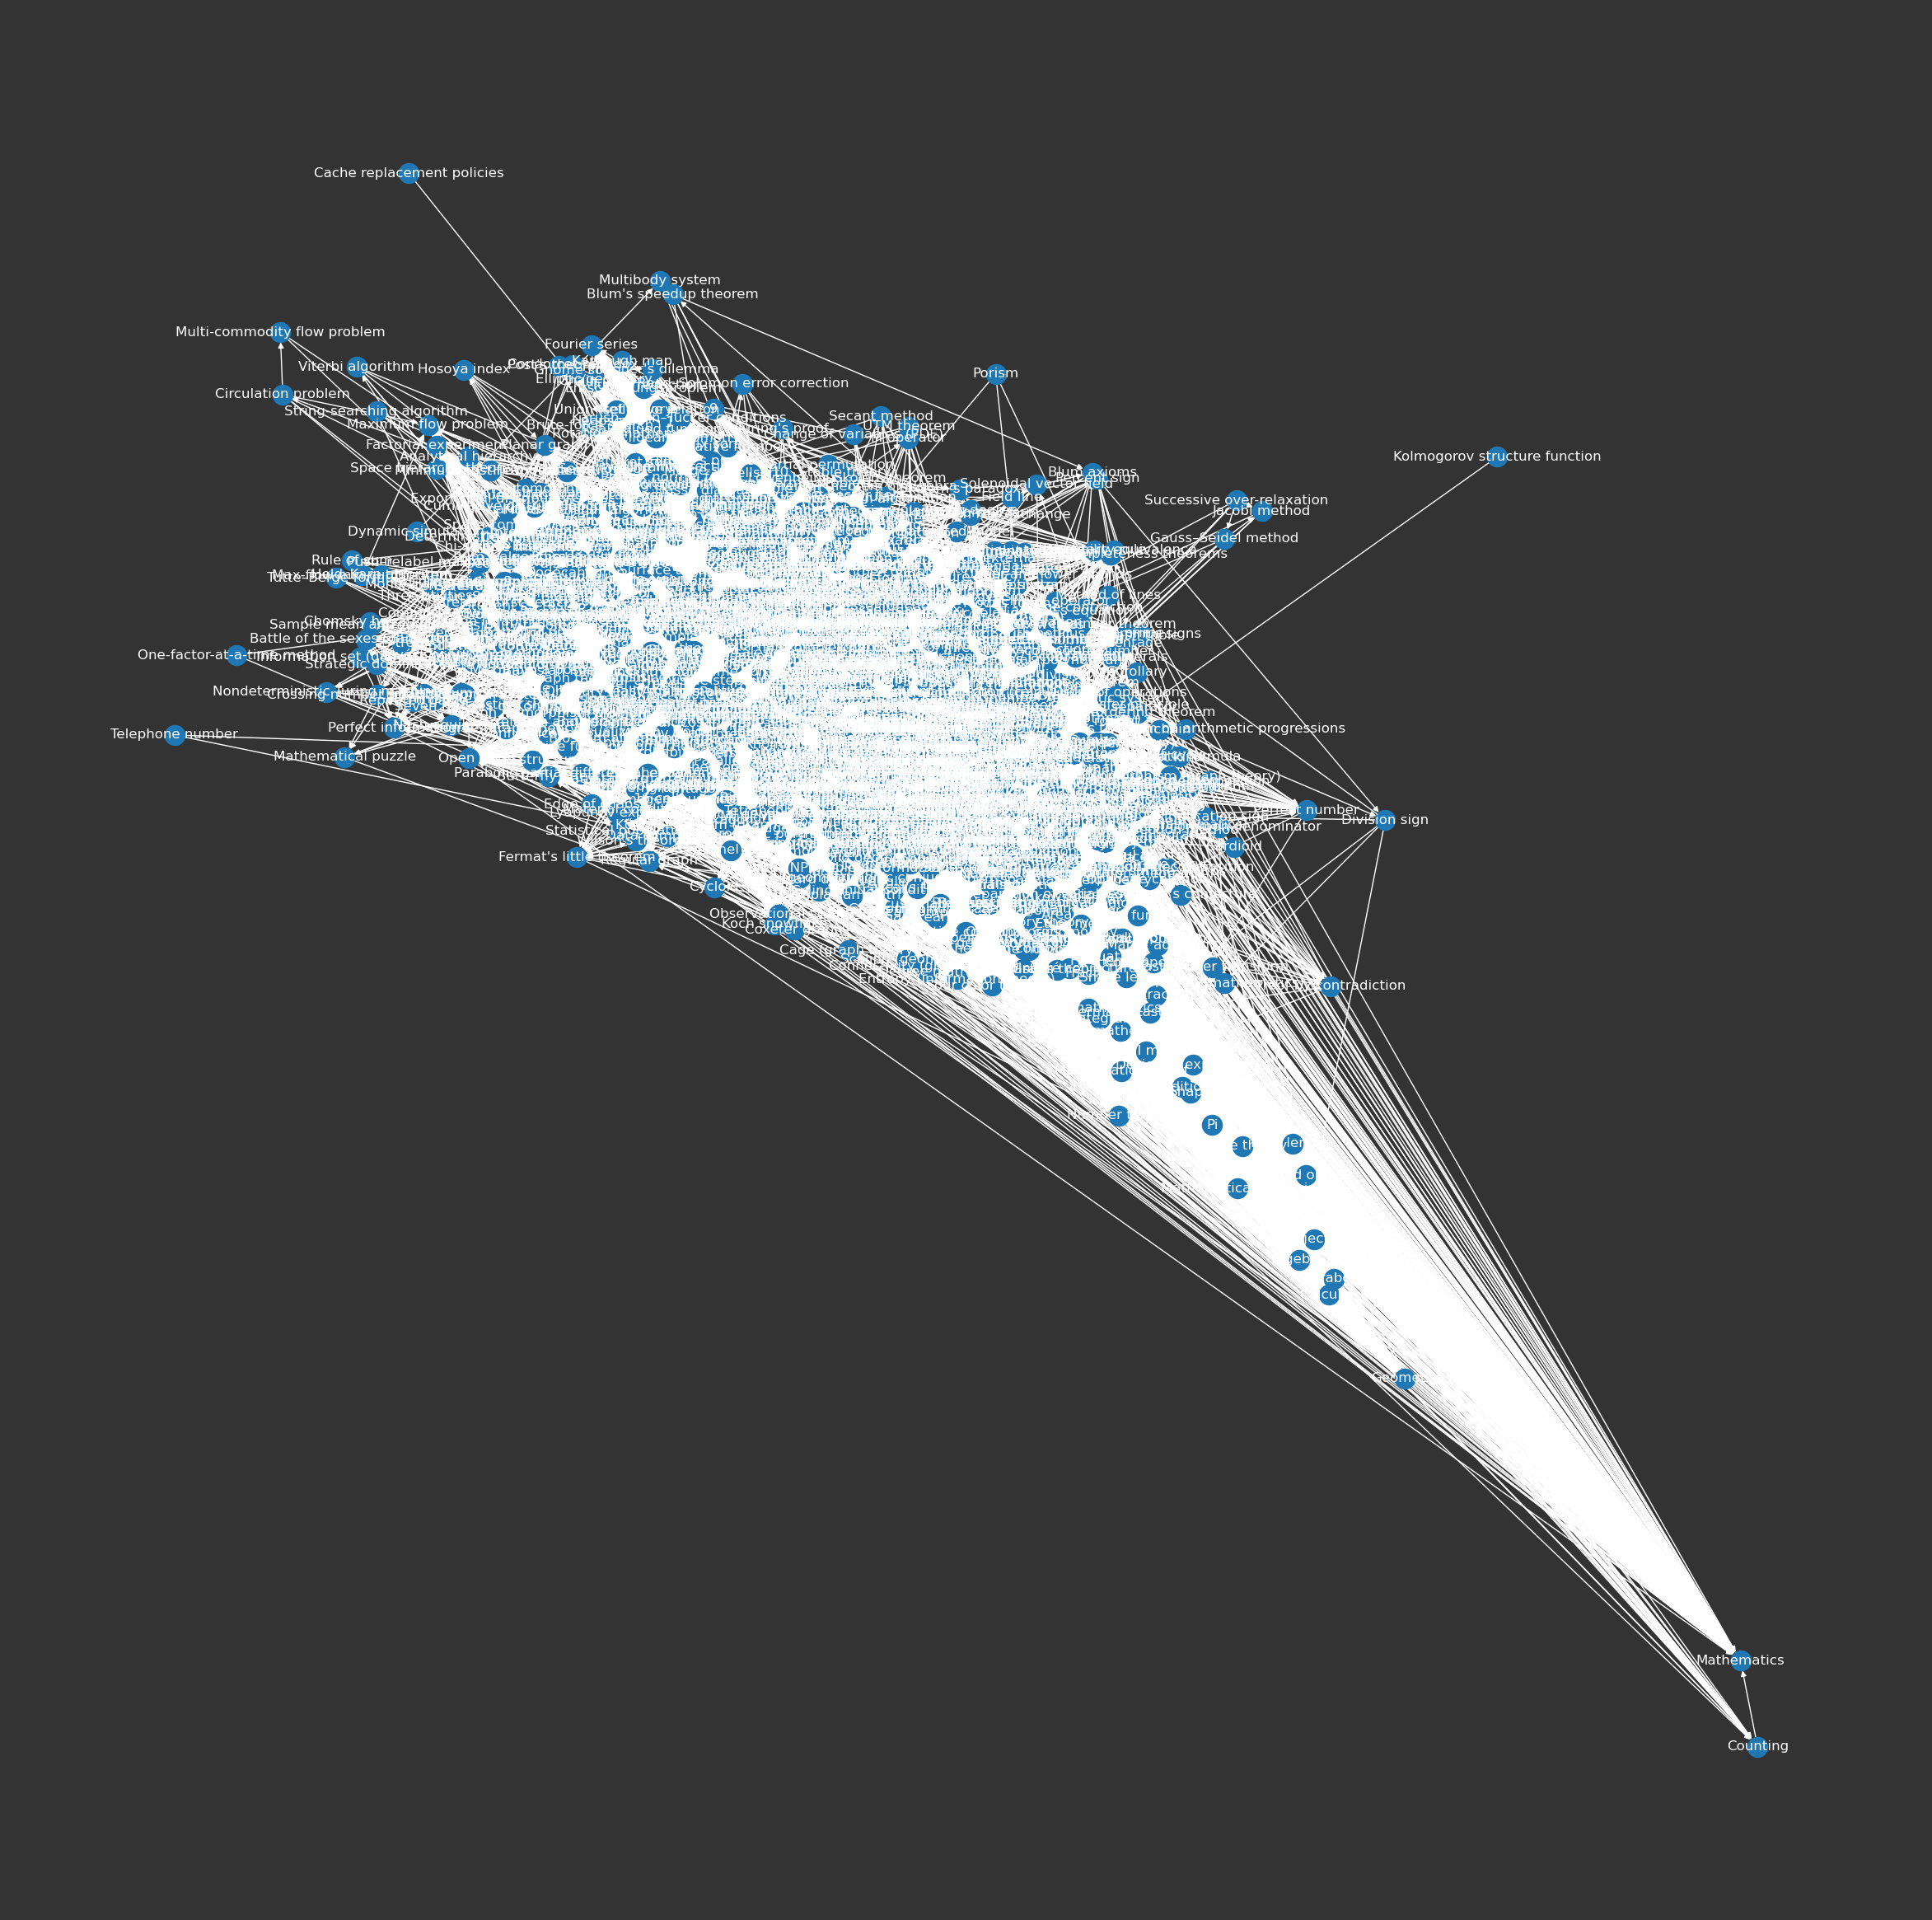
\includegraphics[width=1\textwidth, height=0.4\textheight]{./3ai.png}
            \end{figure}
        \end{minipage}

        \item \begin{minipage}[t]{0.9\textwidth}
            Indegree and Outdegree distributions:
            \begin{figure}[H]
                \centering
                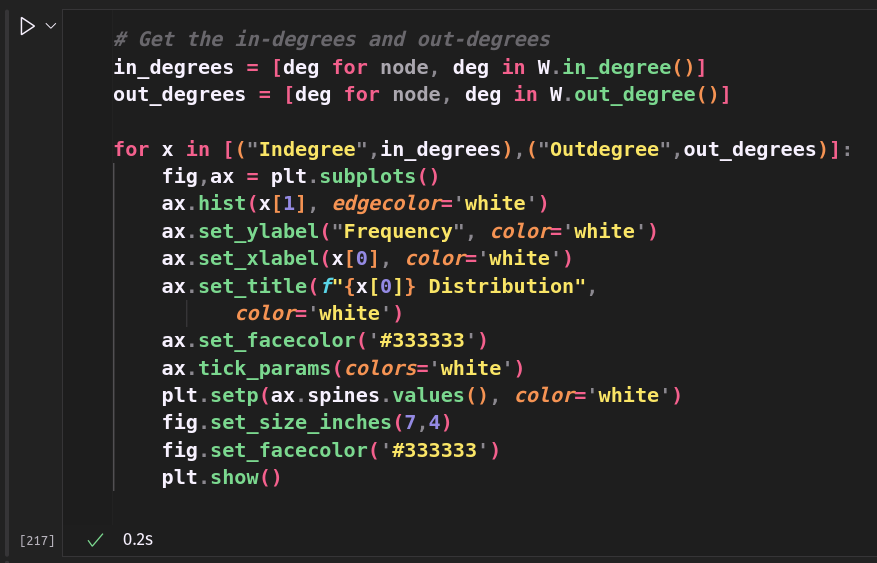
\includegraphics[width=0.8\textwidth, height=0.3\textheight]{./3b.png}
                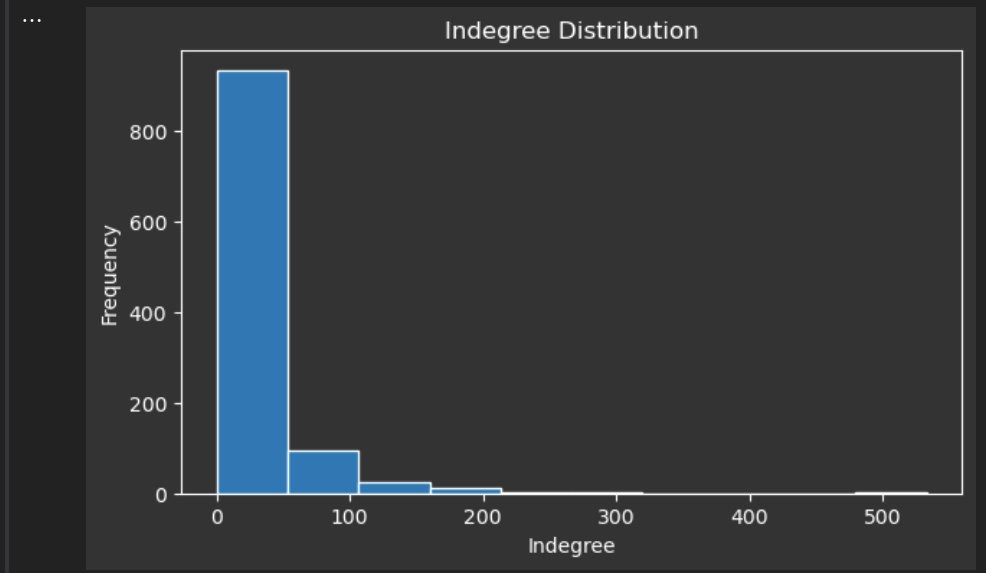
\includegraphics[width=0.8\textwidth, height=0.2\textheight]{./3bi.png}
                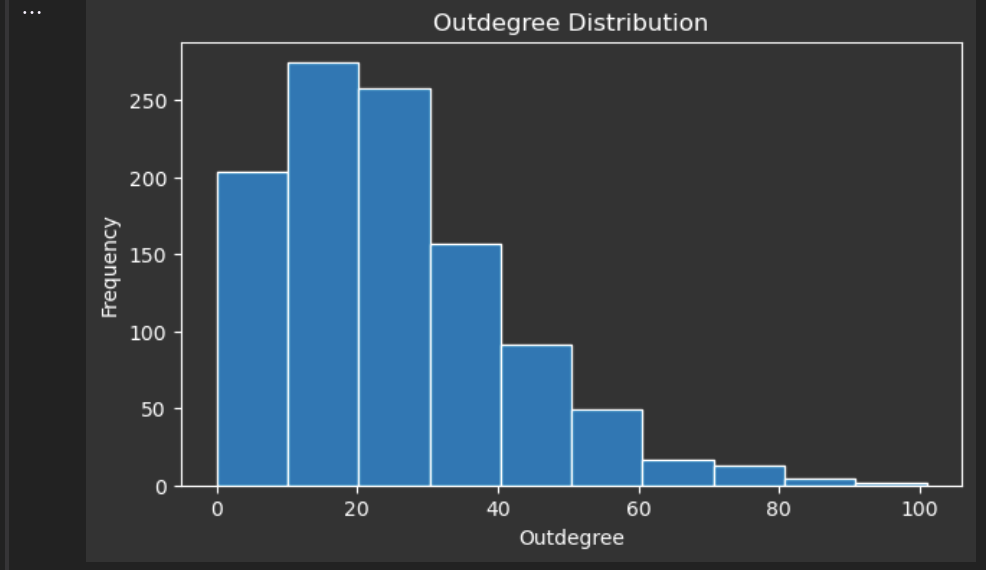
\includegraphics[width=0.8\textwidth, height=0.2\textheight]{./3bii.png}
            \end{figure}

            \begin{enumerate}
                \item[i)]  Only the Indgree distribution follows the power-law.
                \item[ii)] I believe these distributions do make sense. The majority of pages
                           would be linked to by very few other pages while a small number of
                           nodes representing the fundamental concepts in mathematics such as
                           algebra, calculus, geometry, etc... would be linked to by almost
                           everything else. This would create a power law for the indegree
                           distribution.

                           As for the outdegree, we could expect that the majority of topics in
                           math are related to a moderate amount of other topics, the majority
                           of which being in the same core branch. Very few topics would be
                           related to a very large number of other topics and so the right
                           skewed graph for the number of pages a given page links does seem
                           reasonable.
            \end{enumerate}
        \end{minipage}

        \item \begin{minipage}[t]{0.9\textwidth}
            Converting the network to an undirected graph:
            \begin{figure}[H]
                \centering
                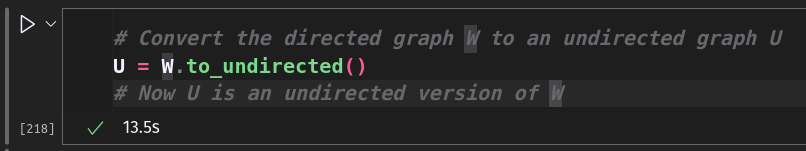
\includegraphics[width=0.8\textwidth, height=0.1\textheight]{./3c.png}
            \end{figure}
        \end{minipage}

        \item \begin{minipage}[t]{0.9\textwidth}
            Top ten betweenness centralities:
            \begin{figure}[H]
                \centering
                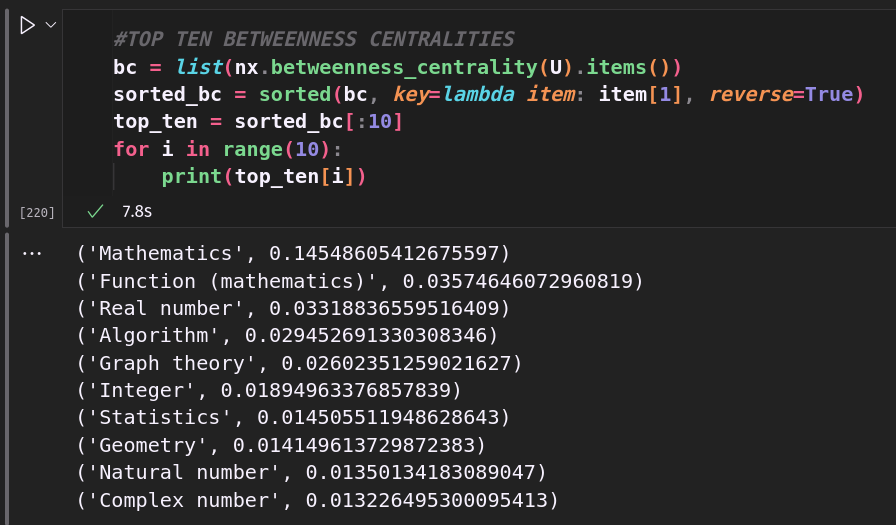
\includegraphics[width=0.8\textwidth, height=0.3\textheight]{./3d.png}
            \end{figure}

            The core branches of mathematics are represented by nodes with the highest
            betweenness centralities. This is logical since every topic in math is categorized
            under one or more of these branches. Consequently, the branches serve as links
            relating seperate topics to each other. This justifies their high betweenness
            centralities.

        \end{minipage}

        \item \begin{minipage}[t]{0.9\textwidth}
            \begin{figure}[H]
                \centering
                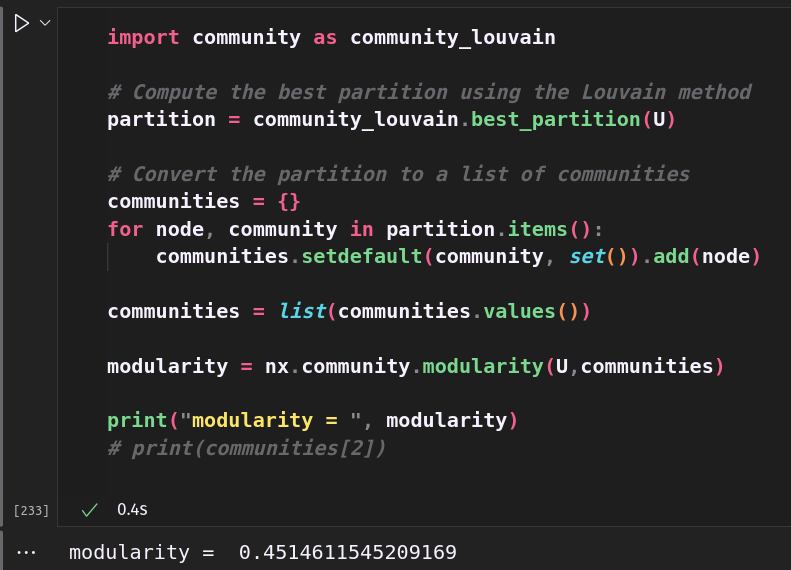
\includegraphics[width=0.8\textwidth, height=0.3\textheight]{./3e.png}
            \end{figure}
            Using the louvain algorithm we find a partition with maximum modularity of approx
            0.451 which indicates good community structure.
        \end{minipage}
        
        \item \begin{minipage}[t]{0.9\textwidth}
            Looking at the third community, we see that the main theme seems to be calculus
            and differential equations.
        \end{minipage}

        \item \begin{minipage}[t]{0.9\textwidth}
            Converting from a directed to undirected graph would be approriate depending on the
            type of analysis being performed. For example, in the context of the math pages graph,
            all topics eventually point back to their containing branch and so converting the edges
            to undirected is an effective way to detect communitites. This is because in both the
            the directed and undirected case, and edge retains its main purpose of depicting
            relation between topics.
        \end{minipage}

    \end{enumerate}


\end{document}